%-------------------------------------------------------------------------------
% potext-reference-guide
%-------------------------------------------------------------------------------
%
% \file        potext-reference-guide.tex
% \library     Documents
% \author      Chris Ahlstrom
% \date        2024-02-08
% \update      2024-04-06
% \version     $Revision$
% \license     $XPC_GPL_LICENSE$
%
%     This document provides LaTeX documentation for the potext library.
%
%-------------------------------------------------------------------------------

\documentclass[
 11pt,
 twoside,
 a4paper,
 final                                 % versus draft
]{article}

%-------------------------------------------------------------------------------
% docs-structure
%-------------------------------------------------------------------------------
%
% \file        docs-structure.tex
% \library     Documents
% \author      Chris Ahlstrom
% \date        2015-04-20
% \update      2024-01-25
% \version     $Revision$
% \license     $XPC_GPL_LICENSE$
%
%     This "include file" provides LaTeX options for a document.
%
%     Note that enumitem is an extension of enumerate, and comes from
%     Debian's texlive-latex-recommended package.
%
%-------------------------------------------------------------------------------

\usepackage{enumitem}         % setting the whitespace between and within lists
\setlistdepth{9}
\setlist{noitemsep}           % spacing within the list

\usepackage{comment}         % For the comment macro
\usepackage{color}            % provide colors?
\usepackage{nameref}          % Provide references by name instead of number
\usepackage[obeyspaces]{url}  % Required for including URLs, ahead of hyperref
\usepackage[colorlinks=true,linkcolor=webgreen,filecolor=webbrown,citecolor=webgreen]{hyperref}
\definecolor{webgreen}{rgb}{0,.5,0}
\definecolor{webbrown}{rgb}{.6,0,0}

\usepackage{ragged2e}         % For underfull boxes in the bibliography
\usepackage{wasysym}          % For smileys
\usepackage{verbatim}         % For the comment macro
\usepackage{amsthm}           % Helps avoid "destination with same
\usepackage[hypcap]{caption}  % make labels point to figure, not the caption
\usepackage[pdftex]{graphicx} % Required for including images
\graphicspath{{images/}}      % Set the default folder for images
\usepackage{float}            % For more control of location of Figures
\usepackage[T1]{fontenc}      % Remove font warnings for textleftbrace, etc.
\usepackage{geometry}         % Page & text layout
\geometry{
  letterpaper,
  top=2.5cm,
  bottom=2.5cm,
  left=2.5cm,
  right=2.5cm
}

% Experimental: remove indent from all paragraphs and set whitespace between
% paragraphs.  These don't work! But see seq66-user-manua.tex lines 80-81.
%
% \usepackage{parskip}
% \setlength{\parindent}{0cm}
% \setlength{\parskip}{2ex plus 0.5ex minus 0.2ex} % whitespace between paragraphs

\usepackage{longtable}        % For making multi-page tables
\usepackage{makeidx}          % For making an index

% Try to reduce the space before or after verbatim sections.
% Doesn't affect the spacing after the verbatim, though.
%
% Fonts sizes are "tiny", "scriptsize", "footnotesize", "small",
% "normalsize", "large", "Large", and "LARGE".

\usepackage{etoolbox}
\makeatletter
\preto{\@verbatim}{\topsep=6pt \partopsep=0pt}
\patchcmd{\@verbatim}
   {\verbatim@font}
   {\verbatim@font\footnotesize}
   {}{}
\makeatother

% Let's try to reduce the size of quotations.

\usepackage{relsize,etoolbox}          % http://ctan.org/pkg/{relsize,etoolbox}
\AtBeginEnvironment{quotation}{\smaller}   % Step font down one size relatively

% For the MIDI Implementation Chart

\usepackage{makecell}

% This package isn't available easily on CentOS:
%
% \usepackage[subtle]{savetrees} % For tightening document vertical spacing

\hypersetup{                  % HYPERLINKS
% draft,                      % Uncomment removes links (e.g. for B&W printing)
 colorlinks=true,
 breaklinks=true,
 bookmarksnumbered,
 urlcolor=webbrown,
 linkcolor=blue,              % RoyalBlue
 citecolor=webgreen,
 pdftitle={},
 pdfauthor={\textcopyright},
 pdfsubject={},
 pdfkeywords={},
 pdfcreator={pdfLaTeX},
 pdfproducer={LaTeX with hyperref and ClassicThesis}
}

% Make an "enumber" style that makes all levels of enumerated lists show
% arabic numerals.

\newlist{enumber}{enumerate}{10}
\setlist[enumber]{nolistsep,label=\arabic*.}

% Make "paragraph" a fourth level, and make it shown in the table of
% contents.

\makeatletter
\renewcommand\paragraph{\@startsection{paragraph}{4}{\z@}%
   {-2.5ex\@plus -1ex \@minus -.25ex}%
   {1.25ex \@plus .25ex}%
   {\normalfont\normalsize\bfseries}}
\makeatother
\setcounter{secnumdepth}{4} % how many sectioning levels to assign numbers to
\setcounter{tocdepth}{4}    % how many sectioning levels to show in ToC

% Provide a way of counting user-interface items without putting them in an
% enumberation.

\newcounter{ItemCounter}

% Makes a numbered paragraph out of an item, and allows two index entries
% for it.

\newcommand{\itempar}[2] {
   \noindent
   \stepcounter{ItemCounter}
   \textbf{\arabic{ItemCounter}. #1.}
   \index{#1}
   \index{#2}
}

% Provides for two forms of an option, as might be shown in a man page.

\newcommand{\optionpar}[2] {
   \textbf{\texttt{#1}} \textbf{\texttt{#2}} \\
   \index{#1}
   \index{#2}
}

% Similar, but with no line break.

\newcommand{\optionline}[2] {
   \textbf{\texttt{#1}} \textbf{\texttt{#2}}
   \index{#1}
   \index{#2}
}

% Now deprecated in preference to \itempar

\newcommand{\settingdesc}[2] {
   \textbf{#1}
   \index{#1}
   \index{#2}
}

% Reference to a configuration file setting

\newcommand{\configref}[3] {
   \index{#1!#2}
   \-\hspace{2cm} \textsl{qseq66.#1}: \texttt{[#2] #3}
}

% Make a full reference to a figure using its number, its name, and its page
% number.  Very useful if you have a hard-copy of the document to deal with.

\newcommand{\figureref}[1] {
   Figure~\ref{#1}
   "\nameref{#1}"
   on page~\pageref{#1}\ignorespaces
}

% Make a full reference to a section using its number, its name, and its page
% number.  Very useful if you have a hard-copy of the document to deal with.

\newcommand{\sectionref}[1] {%
   section~\ref{#1}
   "\nameref{#1}"
   on page~\pageref{#1}\ignorespaces
}

% Make a full reference to a "paragraph"  using its number, its name, and
% its page number.  Very useful if you have a hard-copy of the document to
% deal with.

\newcommand{\paragraphref}[1] {%
   paragraph~\ref{#1}
   "\nameref{#1}"
   on page~\pageref{#1}\ignorespaces
}

% Make a full reference to a table using its number, its name, and its page
% number.  Very useful if you have a hard-copy of the document to deal with.

\newcommand{\tableref}[1] {%
   table~\ref{#1}
   "\nameref{#1}"
   on page~\pageref{#1}\ignorespaces
}

% For lining up enumerated items.  Doesn't really work well, better
% to create a table.

\newcommand{\itab}[1]{\hspace{0em}\rlap{#1}}
\newcommand{\tab}[1]{\hspace{.1\textwidth}\rlap{#1}}

% Change the fragction of the page that can be filled with graphics from 0.7
% to 0.9.

\renewcommand\floatpagefraction{.9}
\renewcommand\dblfloatpagefraction{.9}
\renewcommand\topfraction{.9}
\renewcommand\dbltopfraction{.9}
\renewcommand\bottomfraction{.9}

\raggedbottom                          % avoid excessive vertical justification

%-------------------------------------------------------------------------------
% vim: ts=3 sw=3 et ft=tex
%-------------------------------------------------------------------------------
             % specifies document structure and layout

\usepackage{fancyhdr}
\pagestyle{fancy}
\fancyhead{}
\fancyfoot{}
\fancyheadoffset{0.005\textwidth}
\lhead{Potext Library Reference and Usage}
\chead{}
\rhead{Developer Guide}
\lfoot{}
\cfoot{\thepage}
\rfoot{}

% Removes the many "headheight is too small" warnings.

\setlength{\headheight}{14.0pt}

\makeindex

\begin{document}

\title{Potext Developer Guide 0.2}
\author{Chris Ahlstrom \\
   (\texttt{ahlstromcj@gmail.com})}
\date{\today}
\maketitle

\begin{figure}[H]
   \centering 
   
\includegraphics[scale=0.65]{potext-logo.png}
   \caption*{Pseudo-Greek Transliteration}
\end{figure}

\clearpage                             % moves Contents to next page

\tableofcontents
\listoffigures                         % print the list of figures

% No tables as of now
%
% \listoftables                        % print the list of tables

\parindent 0pt
\parskip 9pt

\rhead{\rightmark}         % shows section number and section name

\section{Introduction}
\label{sec:introduction}

   The \textsl{potext} libraries adopt, refactor, and greatly extend the
   \textsl{tinygettext} library (\cite{tinygettext}).
   The purpose of that library is to provide a lightweight mechanism
   to do translations using the
   \textsl{Portable Object} translation files, \texttt{*.po}, directly.
   Also incorporated are some elements of the
   \textsl{simple-gettext} library (\cite{simplegettext})
   to support handling \textsl{Machine Object} files, \texttt{*.mo}.

   The purpose of the \textsl{Potext} library is to provide \texttt{C++}
   functions that mirror the many functions of \textsl{gettext},
   including 
   \texttt{textdomain()},
   \texttt{bindtextdomain()},
   \texttt{bind\_textdomain\_codeset()},
   \texttt{gettext()},
   \texttt{dgettext()},
   \texttt{ngettext()},
   and others, for translations made via
   \textsl{GNU PO} files and
   \textsl{GNU MO} files.
   In addition, some of the details of \textsl{tinygettext} 
   are wrapped so that, other than marking the text to be translated,
   the translation setup is done by calling a single function in
   \texttt{main()}.

   Our main goal is to make it easy and lightweight to internationalize
   an application while sticking with \textsl{GNU Gettext}
   conventions.
   The \textsl{GNU Gettext} manual (\cite{gettextman}) is an important
   resource used in writing \textsl{Potext}.
   Also important is the source code at
   \texttt{savannah.gnu.org} (\cite{gettextcode}).

   Note that \textsl{Potext} requires the usage of \texttt{C++17}
   and above. It support builds using the \textsl{GNU} and \textsl{Clang}
   compilers.
   It also requires the use of \textsl{Meson 1.1} and above.
   See the \texttt{INSTALL} file.
   \textsl{Windows} support (apart from \textsl{Mingw} and
   \textsl{Cygwin} will be provided, but it is not ready yet.

\subsection{Additions to Tinygettext}
\label{subsec:introduction_additions}

   \begin{itemize}
      \item Re-implementations of \textsl{gettext/libintl}
         functions as a module
         (collection of functions) in the \texttt{po} namespace.
      \item Integration of the functions above with the
         dictionary-manager class.
      \item Support for selecting a domain during the run.
      \item Support for selecting a \texttt{.po/.mo} file directly
         and getting domain information from it.
      \item A new class, \texttt{nlsbindings}, to supplement the
         \texttt{language} class.
      \item Full documentation of architecture and usage.
      \item \textsl{Meson} \texttt{.wrap} files to use \textsl{Potext}
         as a subproject.
         A sample application project is stored in the tar-file noted
         below.
      \item With version 0.2, \textsl{Potext} can also read
         \textsl{GNU} \texttt{.mo} files for more complete
         compatibility with \textsl{GNU Gettext}.
      \item Additional test programs, test \texttt{.po} files,
         test \texttt{.mo} files, and upgrades to existing tests.
   \end{itemize}

   With these additions, \textsl{Potext} should be relatively straightforward
   to use in a new \texttt{C++} application.
   The tar-ball
   \texttt{extras/code/mini-potext-test.tar.xz}
   contains a simple application using \textsl{Potext} as a sub-project
   stored in \textsl{GitHub}..
   Unpack the tar-ball into its own directory
   and build it by running its
   \texttt{work.sh} script.

\subsection{Deletions from GNU Gettext}
\label{subsec:introduction_deletions}

   \begin{itemize}
      \item Locking has been removed from some \texttt{gettext()}-like
         functions; locking can be put back once testing reveals
        it necessary for the use-cases that \textsl{Potext} supports.
      \item Determining if the binary is running SUID root.
   \end{itemize}

   Currently \textsl{Potext} is meant to be set up once during
   the run of an application.
   It currently does not detect changes to the environment variables
   related to localization and character conversions.
   It assumes that once the setup is made, no localization changes
   will be made. Keeps it simple.

\subsection{Code Changes}
\label{subsec:introduction_changes}

   \begin{itemize}
      \item Changed the coding style and naming conventions for
         (perhaps) easier reading..
      \item Use of initializer lists, rather than brute-force
         assignment statements, for initializing various containers.
      \item Use of the \texttt{auto} keyword in declarations and
         \texttt{for}-loops.
      \item Many additional \texttt{using} directives, most hidden
         in the \texttt{po} namespace or in a class declaration..
      \item A few additional helper classes have been added to provide
         new features.
   \end{itemize}

   These changes are meant to make the code easier to read and understand.

\subsection{Future Work}
\label{subsec:introduction_future}

   \begin{itemize}
      \item Hammer on this code in \textsl{Windows}.
      \item Work out the installation process; including \texttt{.po}
         and \texttt{.mo} file
         installation and copying (if desired)
         to the user's configuration directory.
      \item Handle capitals, punctuation, etc. without additional
         \texttt{.po}/\texttt{.mo} entries.
      \item Get the handling of categories (e.g. \texttt{LC\_TIME}) to
         work. However, note that the category is almost always
         \texttt{LC\_MESSAGES}, so this is a low priority.
      \item Handle the "C" locale as discussed below.
      \item Allow for the user to override the character set via the
         \texttt{OUTPUT\_CHARSET} environment variable.
      \item Add support to assist a \textsl{Potext}-using project with the
         installation of the \texttt{.po} files.
   \end{itemize}

   Ignore \texttt{LANGUAGE} and its system-dependent analog if the locale is
   set to "C" because:

   \begin{enumber}
      \item "C" locale uses the ASCII encoding; most international
         messages use non-ASCII characters, which get displayed
         as question marks or as invalid 8-bit characters.
      \item The precise output of some programs in the "C" locale
         is specified by POSIX and should not depend on environment
         variables like \texttt{LANGUAGE}.  Such programs can use
         \texttt{gettext()}.
   \end{enumber}

   Also ignore \texttt{LANGUAGE} and its system-dependent analog if the
   locale is \texttt{C.UTF-8} or \texttt{C.<encoding>}; that's
   the by-design behaviour for \texttt{glibc}, see
   \url{https://sourceware.org/glibc/wiki/Proposals/C.UTF-8}.
   Also look in \texttt{/usr/lib/locale/C.utf8}.

\subsection{Naming Conventions}
\label{subsec:introduction_conventions}

   \textsl{Potext} uses some conventions for naming things in this
   document.

   \begin{itemize}
      \item \texttt{\$prefix}. The base location for installation of
         the application and its ancillary data files on
         \textsl{UNIX/Linux/BSD}:
         \begin{itemize}
            \item \texttt{/usr/}
            \item \texttt{/usr/local/}
         \end{itemize}
      \item \texttt{\$winprefix}. The base location for installation of
         the application and its ancillary data files on \textsl{Windows}.
         \begin{itemize}
            \item \texttt{C:/Program Files/}
            \item \texttt{C:/Program Files (x86)/}
         \end{itemize}
      \item \texttt{\$podir}. The installed location of the \texttt{*.po}
         files.  The directory \texttt{share} (\textsl{Linux}) or
         \texttt{data} (\textsl{Windows}),
         the package-name of the application
         (\texttt{PACKAGE}), and \texttt{po} are concatenated,
         and again the conventions differ between operating systems.
         \begin{itemize}
            \item \texttt{/usr/share/PACKAGE/po/}
            \item \texttt{/usr/local/share/PACKAGE/po/}
            \item \texttt{C:/Program Files/PACKAGE/data/po/}
            \item \texttt{C:/Program Files (x86)/PACKAGE/data/po/}
         \end{itemize}
      \item \texttt{\$home}. The alternate installed
         location of the \texttt{*.po} files.
         Not to be confused with \texttt{\$HOME}, this is
         the standard location for configuration files.
         On a UNIX-style system, it would be \linebreak
         \texttt{\$HOME/.config/appname}.
         The files would be put into a \texttt{po} subdirectory here.
      \item \texttt{\$localedir}. The installed
         location of the \texttt{*.mo} files.
         The directory \texttt{share} (\textsl{Linux})
         or \texttt{data} (\textsl{Windows}),
         the package-name of the application
         (\texttt{PACKAGE}), and \texttt{locale} are concatenated.
         The conventions for \textsl{Linux} versus \textsl{Windows}
         differ as a matter of historical interest:
         \begin{itemize}
            \item \texttt{/usr/share/PACKAGE/locale/}
            \item \texttt{/usr/local/share/PACKAGE/locale/}
            \item \texttt{C:/Program Files/PACKAGE/data/locale/}
            \item \texttt{C:/Program Files (x86)/PACKAGE/data/locale/}
         \end{itemize}
            At present, \textsl{Potext} does not support directories of
            \texttt{.mo} files. It might, in the future.
      \item \texttt{\$modir} and \texttt{LC\_MESSAGES}.
            A more common convention for
            \texttt{*.mo} files on \textsl{UNIX} is to put them in
         \begin{itemize}
            \item \texttt{/usr/share/locale/<language>/LC\_MESSAGES/PACKAGE.mo}
            \item \texttt{/usr/local/share/locale/<language>/LC\_MESSAGES/PACKAGE.mo}.
         \end{itemize}
   \end{itemize}

   Currently, the \textsl{Potext} library uses only the \texttt{*.po} files.
   In the future it might also handle \texttt{*.mo} files.
   Also note that various applications differ in the exact location of their
   translation files.

\subsection{Home Potext Configuration}
\label{subsec:introduction_home_potext_configuration}

   The \textsl{Potext} library also supports installing the
   \texttt{*.po} and \texttt{*.mo} translation files in the
   user's configuration area.
   The conventions we use are:

   \begin{itemize}
      \item \texttt{\$home}. The location where \texttt{PACKAGE} installs,
         creates, or copies its configuration files.
         Do not confuse it with \texttt{\$HOME},
         although \texttt{\$home} is in
         \texttt{\$HOME/.config/PACKAGE}.
         The \texttt{*.po} files are stored in
         \texttt{\$HOME/.config/PACKAGE/po}.
      \item \texttt{\$winhome}. This location is different for
         \textsl{Windows}:
         \texttt{C:/Users/user/AppData/Local/PACKAGE}.
         Again, the \texttt{*.po} files are in a
         subdirectory called \texttt{po}.
   \end{itemize}

   Also, for reference, we mention some of the files used by
   \textsl{GNU Gettext}.

   \begin{itemize}
      \item \texttt{PACKAGE.pot}, created by \texttt{xgettext}.
      \item \texttt{LANG.po}, created by \texttt{msgmerge},
         copying \texttt{PACKAGE.pot}, or by editing.
      \item \texttt{LANG.gmo}, created by \texttt{msgfmt}.
      \item For installed packages, see
         \texttt{\$prefix/locale/LANG/PACKAGE.mo}.
      \item Or see
         \texttt{\$prefix/locale-langpack}.
         \texttt{LC\_category} (e.g. \texttt{LC\_NUMERIC}).
      \item \texttt{LANG/PACKAGE.po}, reverse engineered from
         \texttt{PACKAGE.mo} by \texttt{msgunfmt}.
   \end{itemize}

   Also refer to the \textsl{Python} packages \textsl{polib} (\cite{polib})
   and \textsl{poedit} (\cite{poedit}).

%----------------------------------------------------------------------------
% Additional Chapters
%----------------------------------------------------------------------------

%-------------------------------------------------------------------------------
% usage
%-------------------------------------------------------------------------------
%
% \file        usage.tex
% \library     Documents
% \author      Chris Ahlstrom
% \date        2024-03-19
% \update      2024-03-22
% \version     $Revision$
% \license     $XPC_GPL_LICENSE$
%
%     Provides a description of how to use potext in an application.
%
%-------------------------------------------------------------------------------

\section{Potext Usage in Applications}
\label{subsec:potext_usage}

   This section briefly covers the usage of \textsl{Potext} in an
   application.
   A real sample is included in \texttt{library/tests/hellopotext.cpp}
   (see \sectionref{subsec:potext_hello_potext}).
   A small sample application showing the usage of
   \textsl{Potext} as a \textsl{Meson subproject} in a completely
   separate application project is
   contained in:

   \begin{verbatim}
      extras/code/mini-potext-test.tar.xz
   \end{verbatim}

   Unpack this file in its own directory and check it out.

\subsection{Main Module Using Potext}
\label{subsubsec:potext_usage_main}

   The first thing is to add the following header file
   to the module defining the \texttt{main()} function.

   \begin{verbatim}
      #include "po/potext.hpp"      // includes "po/gettext.hpp"
   \end{verbatim}

   For clarity, \texttt{potext.hpp} is better, but it does include
   an extra header file.

   If \textsl{Potext} support is optional for the project, then do
   something like this; \texttt{PROJECT\_USE\_POTEXT}
   is a macro optionally defined when configuring the project build.

   \begin{verbatim}
      #if defined PROJECT_USE_POTEXT
      #include "po/potext.hpp"   // includes "po/gettext.hpp"
      else
      #define _(str)             (str)
      #define N_(str)            str
      #endif
   \end{verbatim}

   An application using "gettext" internationaliztion generally needs
   to call \texttt{setlocale()},
   \texttt{textdomain()}, and \texttt{bindtextdomain()}.
   The following function wraps up these functions in one call.

   \begin{verbatim}
      std::string init_app_locale
      (
          const std::string & arg0,
          const std::string & pkgname,
          const std::string & domainname,
          const std::string & dirname,
          int category
      )
   \end{verbatim}

   \texttt{arg0}.
   The path-name by which the program was called. This information
   can determine more precisely where installed \texttt{.po} files might be
   stored.

   \texttt{pkgname}.
   The name of the PACKAGE, which can be the short name for
   the program, such as "helloworld".

   \texttt{domainname}.
   The base name of a message catalog, such as "en\_US".
   It must consist of characters legal in filenames.
%  We might support a value of "0" to reset the domain to
%  "messages".
   An application might want to use its
   package name, such as "helloworld", for the domain name.
   If empty, then the environment variable \texttt{TEXTDOMAIN} is used.
   If that's empty, then \texttt{LC\_ALL} is used.
   If that's empty, then \texttt{LC\_MESSAGE} is used.
   Lastly, if that's empty, then \texttt{LANG} is used.

   \texttt{dirname}.
   Provides the name of the \texttt{LOCALEDIR}.
   The standard search directory is \texttt{/user/share/locale}.
   If empty, then the environment variable
   \texttt{TEXTDOMAINDIR} is used.
   If the name is "user", then the \texttt{.po} files are searched
   for in \texttt{/home/user/.config/package/} or
   \texttt{C:/Users/user/AppData/Local}, instead of some
   place in the system.

   \texttt{category}.
   The area that is covered, such as
   \texttt{LC\_ALL}, \texttt{LC\_MONETARY}, and \texttt{LC\_NUMERIC}.
   The default value selects \texttt{LC\_ALL}.

   The following calls are made for the setup:

   \begin{enumber}
      \item \texttt{std::setlocale()} sets the application's current
         category and locale.
         The category is \texttt{LC\_ALL} by default, and the locale
         is empty, so that the locale parts are modified according to
         environment variables.
      \item \texttt{po::set\_locale\_info()} sets up the domain name
         and the locale directory name. If empty, the
         environment variables discussed above are used.
         In addition, it is determined if the locale directory
         is a system directory, the user's configuration directory,
         or some arbitrary directory containing \texttt{.po} files.
      \item \texttt{po::init\_lib\_locale()} first
         asks the dictionary-manager (see 
         \sectionref{sec:potext_architecture})
         to add all of the dictionaries (po files) in that directory
         to the list of selectable dictionaries, making one
         of them the default dictionary.
         Then the reimplementation of the \texttt{bindtextdomain()}
         is called to create a new domain-to-directory binding, and
         it is inserted into a container.
         This container supports looking up the locale directory
         associated with a domain.
% We need to see if we really use nlsbindings!!!!!
      \item \texttt{po::textdomain()}
         This function sets the current domain for the dictionary
         manager to use.
   \end{enumber}

\subsection{Marking a Module for Translation}
\label{subsubsec:potext_usage_marking}

   The basic usage to \textsl{Potext} is essentially identical to
   that of \textsl{GNU Gettext}, except that (currently) only
   \texttt{.po} files are used directly.

   Add the following header file.

   \begin{verbatim}
      #include "po/potext.hpp"      // includes "po/gettext.hpp"
   \end{verbatim}

   Mark each translatable string as usual, using the
   \texttt{\_()} macro:

   \begin{verbatim}
      std::string errmsg = _("Unknown system error");
   \end{verbatim}

   That macro hides a call to \texttt{po::gettext()}.
   Additional "get-text" functions are listed in the table in the
   following section:
   \sectionref{subsec:gettext_module}.

\subsection{Creating the .po Files}
\label{subsubsec:potext_usage_creating_po_files}

   After marking the files that will provide translations, they must be
   processed to extract the marked strings for translation.
   For example:
   
   \begin{verbatim}
      $ xgettext test_helpers.cpp --keyword="_" --output="es.po"
   \end{verbatim}

   The result is an untranslated template, \texttt{es.po}.

   \begin{verbatim}
      # SOME DESCRIPTIVE TITLE.
      # Copyright (C) YEAR THE PACKAGE'S COPYRIGHT HOLDER
      # This file is distributed under the same license as the PACKAGE package.
      # FIRST AUTHOR <EMAIL@ADDRESS>, YEAR.
      #
      #, fuzzy
      msgid ""
      msgstr ""
      "Project-Id-Version: PACKAGE VERSION\n"
      "Report-Msgid-Bugs-To: \n"
      "POT-Creation-Date: 2024-03-20 06:53-0400\n"
      "PO-Revision-Date: YEAR-MO-DA HO:MI+ZONE\n"
      "Last-Translator: FULL NAME <EMAIL@ADDRESS>\n"
      "Language-Team: LANGUAGE <LL@li.org>\n"
      "Language: \n"
      "MIME-Version: 1.0\n"
      "Content-Type: text/plain; charset=CHARSET\n"
      "Content-Transfer-Encoding: 8bit\n"

#: test_helpers.cpp:79
      msgid "output"
      msgstr ""
       . . .
   \end{verbatim}

   The next step is to edit this file appropriately, as in the following
   snippet:

   \begin{verbatim}
      # Mensajes en español para test_helpers.
      # Copyright (C) 2024 Potext Software Foundation Inc.
      # This file is distributed under the same license as the test_helpers package.
      # Chris Ahlstrom <ahlstromcj@gmail.com>, 2024.
      msgid ""
      msgstr ""
      "Project-Id-Version: Potext test_helpers 0.1.0\n"
      "Report-Msgid-Bugs-To: ahlstromcj@gmail.com\n"
      "POT-Creation-Date: 2023-09-18 22:55+0200\n"
      "PO-Revision-Date: 2024-03-20 17:08+0200\n"
      "Last-Translator: Google Translate <translate.google.com>\n"
      "Language-Team: Spanish <es@tp.org.es>\n"
      "Language: es\n"
      "MIME-Version: 1.0\n"
      "Content-Type: text/plain; charset=UTF-8\n"
      "Content-Transfer-Encoding: 8-bit\n"
      "X-Bugs: Report translation errors to the Language-Team address.\n"
      "Plural-Forms: nplurals=2; plural=(n != 1);\n"

      #: test_helpers.cpp:79
      msgid "output"
      msgstr "producción"
       . . .
   \end{verbatim}

   In the project tree, create a \texttt{po} directory and move the
   \texttt{.po} file to it.

   Note that the \textsl{GNU Gettext} manual (\cite{gettextman}) (in chapter
   6) describes many more facets (heh heh) to the creation and manipulation
   of \texttt{.po} files.

\subsection{Installing the .po Files}
\label{subsubsec:potext_usage_installing_po_files}

   The installation process for the project should include installing the
   \texttt{.po} files.
   Where to install them in the system, if desired?
   It does not quite make sense to store them in a place like

   \begin{verbatim}
      /usr/local/share/locale/LL/LC\_MESSAGES}
   \end{verbatim}

   because that contains \texttt{.mo} files (and some \textsl{Qt}
   \texttt{.qm} files!).

   We would suggest something like
   \texttt{/usr/local/share/po/PACKAGE}.
   We should provide support in \textsl{Potext} for that.
   Once \textsl{Potext} supports parsing \texttt{.mo} files,
   the usual processes and location can be used.
   Future stuff.

   The project, once installed, can also, if desired, copy
   the relevant language file to the user's configuration directory,
   \texttt{/home/user/.config/package/} or
   \texttt{C:/Users/user/AppData/Local} at the first run, and use it
   there.

%-------------------------------------------------------------------------------
% vim: ts=3 sw=3 et ft=tex
%-------------------------------------------------------------------------------

%-------------------------------------------------------------------------------
% architecture
%-------------------------------------------------------------------------------
%
% \file        architecture.tex
% \library     Documents
% \author      Chris Ahlstrom
% \date        2024-03-07
% \update      2024-04-06
% \version     $Revision$
% \license     $XPC_GPL_LICENSE$
%
%     Provides a description of the classes and modules of this library.
%
%-------------------------------------------------------------------------------

\section{Potext Architecture}
\label{sec:potext_architecture}

   This section provides a walk-through of the architecture
   of the \textsl{Potext} library.
   Much of the architecture is similar to \textsl{Tinygettext}
   (\cite{tinygettext}), but
   there are some important changes and additions.
   Some notes about the classes and documentation:

   \begin{itemize}
      \item All classes and free functions are wrapped in the
         \texttt{po} namespace.
      \item The macro \texttt{\_()} that normally wraps \textsl{GNU} function
         \texttt{gettext()} here wraps the \textsl{Potext} function
         \texttt{po::gettext()}.
      \item The related "gettext" functions are redefined in terms of
         \textsl{Potext} functions.
      \item In the diagrams, for the function parameters, we use
         "std::string", rather than "const std::string \&" for brevity in the
         diagrams.
      \item Not every attribute or function is described. Some groups of
         items include \texttt{\_xxxx\_} to represent a number of similar
         functions.
      \item The copy constructors, principal assignment operators, and
         destructors are not described. See the header files to see
         if they are \texttt{default}, \texttt{delete}, or defined.
   \end{itemize}

   First, the big picture.

\begin{figure}[H]
   \centering 
   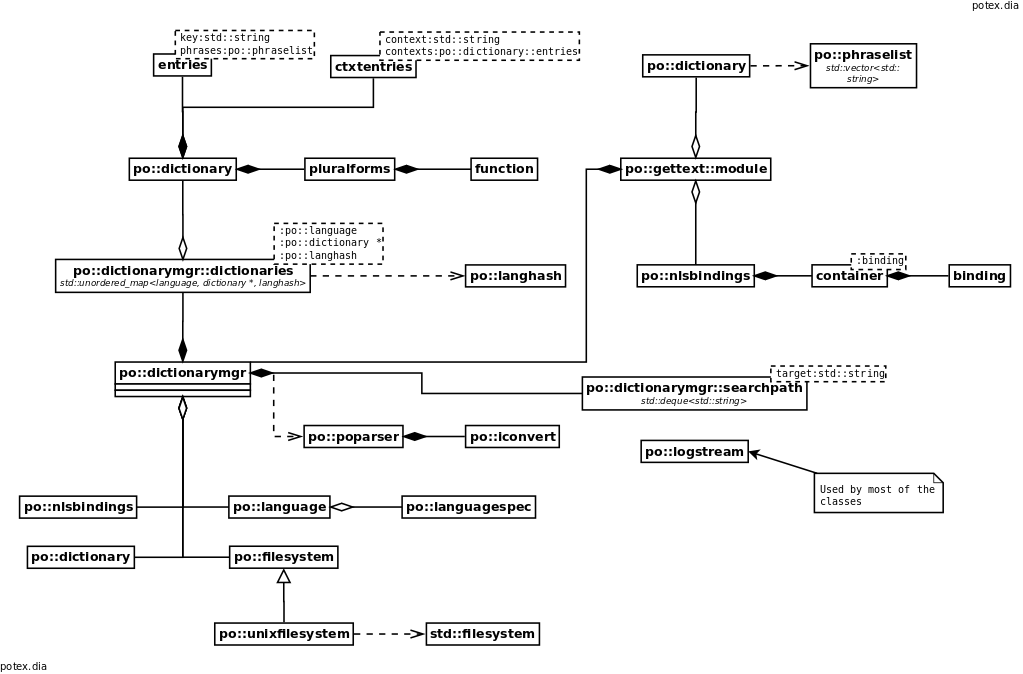
\includegraphics[scale=0.65]{potext.png}
   \caption{Potext "Big Picture" Architecture}
   \label{fig:potext}
\end{figure}

   The most important part of \textsl{Potext} is the
   \texttt{dictionary} class.
   It is filled by the \texttt{po::poparser::parse()} function,
   which takes a \texttt{.po} file and fills a dictionary object
   with a set of message strings and their translations.
   It also includes plural forms from the \texttt{.po} file to
   translate plural messages using "plural" functions.
   Each dictionary includes the message entries and context entries.
   For a description of the \texttt{.po} file, see
   the \textsl{GNU Gettext} manual (\cite{gettextman}).

   The \texttt{dictionarymgr} class handles one or more dictionaries.
   It has been augmented to hold a new \texttt{nlsbindings} class toion
   provided support for \texttt{bindtextdomain} and \texttt{textdomain},
   which are \textsl{not} provided by \textsl{Tinygettext}.

   The \texttt{dictionarymgr}'s additional member functions are used
   to implement the free functions in the \texttt{gettext} module, such
   as \texttt{gettext()} and \texttt{dgettext()},
   etc.
   The \texttt{gettext} module is an addition to \textsl{Potext} to
   make it easy to switch from \textsl{Gettext} to \textsl{Potext}.

   The \texttt{language} class supports the various parts of
   a domain name: language, country, modifier, long name, and the
   long name localized.

   Parsing \texttt{.po} files is facilitated by the various file-system
   classes. Each \texttt{.po} file results in the creation of a dictionary.

   The \texttt{poparser} class supports reading and parsing a
   \texttt{.po} file to create a \texttt{dictionary}.
   It inherits some common code from the
   \texttt{pomoparserbase} class.

   The \texttt{moparser} class supports reading and parsing a
   \texttt{.mo} file to create a \texttt{dictionary}.
   It also inherits some common code from the
   \texttt{pomoparserbase} class.

   The \texttt{iconvert} class supports converting the translations
   to another codeset (besides \texttt{UTF-8}) when creating the
   dictionaries.

   The \texttt{logstream} class supports internal error logging,
   but can also be used by an application.

   These classes are discussed in more detail in the following sections.

\subsection{Logstream Class}
\label{subsec:potext_logstream_class}

   The \texttt{po::logstream} class is a reimplementation of the
   \texttt{tinygettext::Log} class.

\begin{figure}[H]
   \centering 
   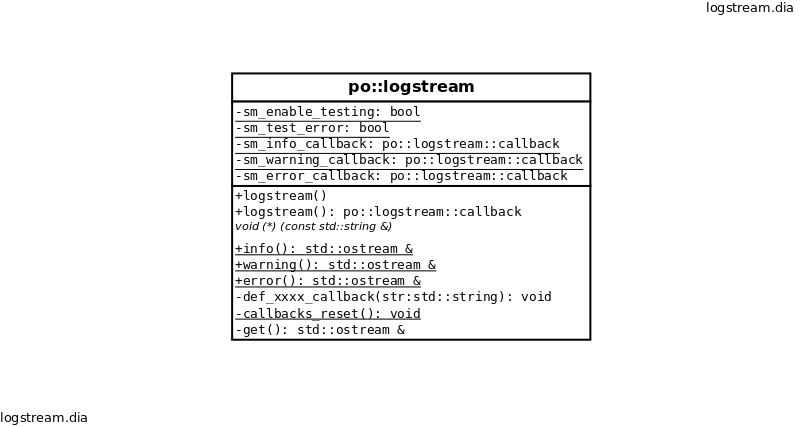
\includegraphics[scale=0.80]{logstream.png}
   \caption{Log Stream (po::logstream)}
   \label{fig:potext_logstream}
\end{figure}

   The \texttt{po::logstream} class provides \texttt{std::ostream}
   objects for emitting errors, warnings, and information messages.
   It also provides the ability to set a callback function to
   change how the messages are emitted.
   It is used internally for writing status to the console.
   It can also be used by an application, but ...

   ... An interesting issue that we have not yet figured out is
   illustrated by the test application \texttt{hellopotext}.
   When run, all of the messages written to \texttt{std::cout}
   appear first, including the final message "SUCCESS".
   Then all of the messages logged during setup and translation in the
   \textsl{Potext} library appear when \texttt{hellopotext}
   is \textsl{exiting}.

\subsection{Dictionary Manager Class}
\label{subsec:potext_dictionarymgr_class}

   The \texttt{po::dictionarymgr} class is a reimplementation of the
   \texttt{tinygettext::dictionary\_manager} class.
   It contains an \texttt{std::unordered\_map} of
   shared pointers to \texttt{dictionary} objects, keyed by
   \texttt{language} objects which are searched using
   \texttt{operator ()} hash function in a \texttt{po::langhash}
   structure.

   Currently, \textsl{Potext} does not do anything special with the
   \texttt{searchpath} deque.

% TODO
% Add the new get_dictionary() function to the diagram.
% TODO

\begin{figure}[H]
   \centering 
   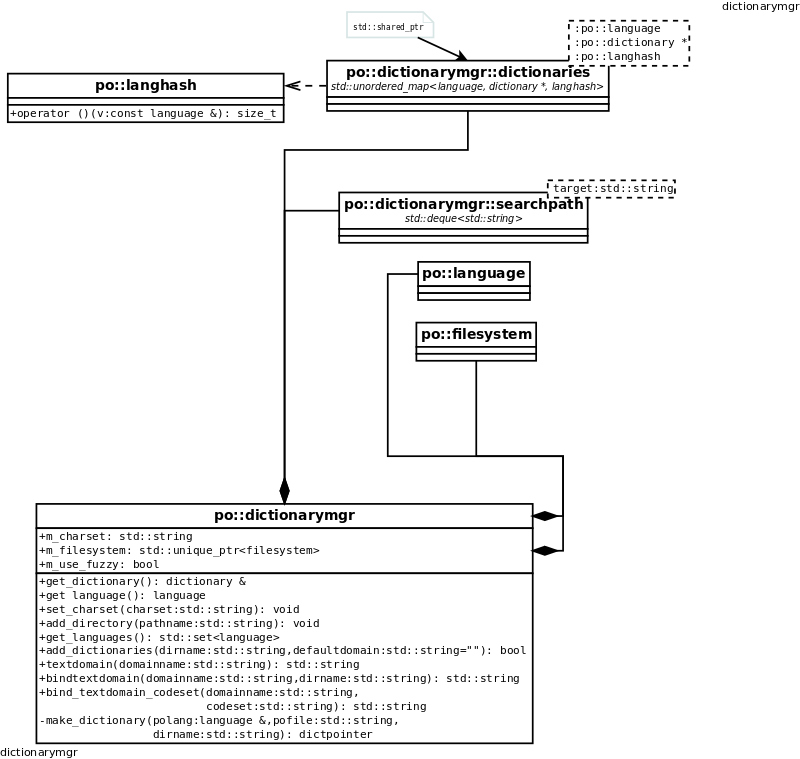
\includegraphics[scale=0.80]{dictionarymgr.png}
   \caption{Dictionary Manager (po::dictionarymgr)}
   \label{fig:potext_dictionarymgr}
\end{figure}

   In \textsl{Tinygettext}, the \texttt{dictionary\_manager} class 
   coordinated multiple locale directories and the selection of
   a particular \texttt{dictionary} for a translation.

   \textsl{Potext}'s \texttt{dictionarymgr}
   currently handles only one directory, but it
   adds support for domain-binding and for actually using translation
   functions that accept a domain parameter.
   The new functions are described next.

   \begin{itemize}
      \item \texttt{get\_bindings()}. This function returns an
         \texttt{nlsbindings} class reference that contains a list of domain
         names with the names of the directory and the character-set
         for each domain.
         The \texttt{nlsbindings} class provides the set-binding functions
         needed by the following new functions.
      \item \texttt{add\_dictionaries()}.
         This function scans a directory for \texttt{.po} files
         and creates a \texttt{dictionary} for each one.
      \item \texttt{make\_dictionary()}.
         This helper function opens a file using \texttt{std::filesystem}
         It then creates an \texttt{std::shared\_ptr} for a new
         \texttt{dictionary} and calls the static function
         \texttt{po::poparser::parse\_po\_file()}.
         Then it calls \texttt{po::nlsbindings::set\_binding\_values()}
         to create a corresponding binding object.
      \item \texttt{textdomain()}.
         This function sets the current domain to the given domain name.
         It is used in the \texttt{gettext} module to
         implement the \texttt{textdomain()} function.
      \item \texttt{bindtextdomain()}.
         This function associates a domain name with a locale directory
         in which to find the \texttt{.po} file.
         It is used in the \texttt{gettext} module to
         implement the \texttt{bindtextdomain()} function.
      \item \texttt{bind\_textdomain\_codeset()}.
         This function associates a domain name with a character-set to
         use in converting messages.
         It is used in the \texttt{gettext} module to
         implement the \texttt{bind\_textdomain\_codeset()} function.
      \item \texttt{get\_dictionary()}.
   \end{itemize}

\subsection{Pomoparserbase Class}
\label{subsec:potext_pomoparserbase_class}

   As of version 0.2, some common functionality has been moved into
   this base class.

\begin{figure}[H]
   \centering 
   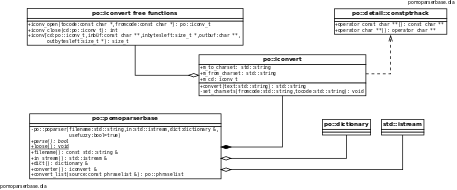
\includegraphics[scale=0.4]{pomoparserbase.png}
   \caption{PO/MO Parser Base (po::pomoparserbase)}
   \label{fig:potext_pomoparserbase}
\end{figure}

   TODO

\subsection{Poparser Class}
\label{subsec:potext_poparser_class}

   The \texttt{po::poparser} class is a reimplementation of the
   \texttt{tinygettext::POParser} class.

\begin{figure}[H]
   \centering 
   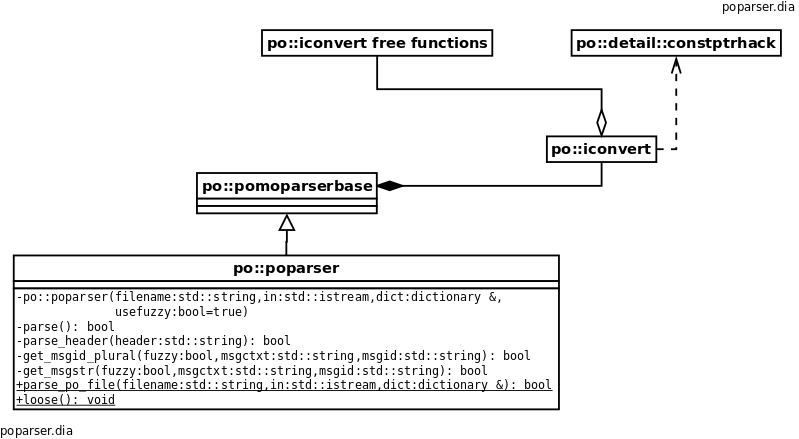
\includegraphics[scale=0.4]{poparser.png}
   \caption{PO Parser (po::poparser)}
   \label{fig:potext_poparser}
\end{figure}

   The \texttt{poparser} "connects" a \texttt{.po} file, an input stream,
   and a \texttt{dictionary} object in order to populate the dictionary with
   plural forms, set the character-set, and use it (if needed) to convert the
   translated message string to the character-set,
   The static function \texttt{po::poparser::parse\_po\_file()} is called to
   create a temporary \texttt{poparser} and use it to
   read a file and fill in an empty \texttt{dictionary}.

   The \texttt{po::poparser::get\_string\_line()} function handles the
   main task of parsing a line from the \texttt{.po} file and deciding
   what to do with it.

   The \texttt{po::poparser::get\_msgstr} function adds a message (which might
   be converted to a specified character-set) to the dictionary.

   The \texttt{po::poparser::get\_msgid\_plural()} adds a plural form
   (see \sectionref{subsec:potext_pluralforms_class})
   or a contextual translation to the dictionary.

%  We need to follow up and make sure that each translation in the list of
%  translations is converted to a specified character-set if applicable.

   The \texttt{po::poparser} class uses the \texttt{po::iconvert} class
   to convert the string translation to the desired character-set.
   The \texttt{po::iconvert} class is a reimplementation of the
   \texttt{tinygettext::IConv} class.
   Note that it defines the \texttt{po::iconv\_t} type.

\subsection{Moparser Class}
\label{subsec:potext_moparser_class}

   The \texttt{po::moparser} class is based on \texttt{pomoparserbase},
   and adds the ability to parse \texttt{.mo} files.
   \texttt{tinygettext::POParser} class.

\begin{figure}[H]
   \centering 
   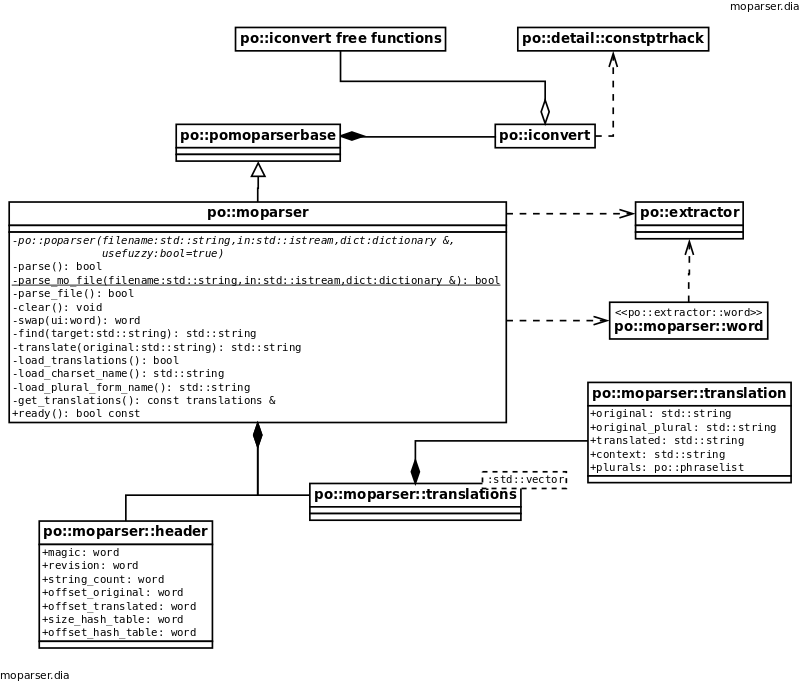
\includegraphics[scale=0.4]{moparser.png}
   \caption{MO Parser (po::moparser)}
   \label{fig:potext_moparser}
\end{figure}

   The \texttt{moparser} "connects" a \texttt{.mo} file, an input stream,
   and a \texttt{dictionary} object in order to populate the dictionary with
   plural forms, set the character-set, and use it (if needed) to convert the
   translated message string to the character-set,
   The static function \texttt{po::moparser::parse\_mo\_file()} is called to
   create a temporary \texttt{moparser} and use it to
   read a file and fill in an empty \texttt{dictionary}.

   The format of the \texttt{.mo} file is described in the \texttt{moparser}
   module's top banner. The format is dissected and described further in the
   files
   \texttt{library/tests/mo/es/newt.hex} and
   \texttt{library/tests/mo/de/helloworld.hex}.

   Note the \texttt{moparser::header} structure, which provides
   the layout of the first few words in the \texttt{.mo} file.
   Each \texttt{translation} structure holds the "original" message ID,
   the "original plural" message ID, the context (if specified),
   the translated singular string, and a list of plural forms (if specified).

   The \texttt{moparser} class gets the character-set name and the
   plural-forms description by searching for the key strings to find them.
   It then searches for original singular strings, original
   plural strings, context strings, and the list of plural translations.
   These items are stored in a vector of translations, which is later
   used to populate a \texttt{dictionary}.

   The process of the binary data is facilitated by the \texttt{extractor}
   class discussed in the next section.

\subsection{Extractor Class}
\label{subsec:potext_extractor_class}

   This new class is used internally in the parsing of \texttt{.mo}
   files. It encapsulates some tricky binary data extraction
   so that the \texttt{moparser} class is less complex than otherwise.
   The binary data is represented by a string, which is loaded by the
   constructor.

\begin{figure}[H]
   \centering 
   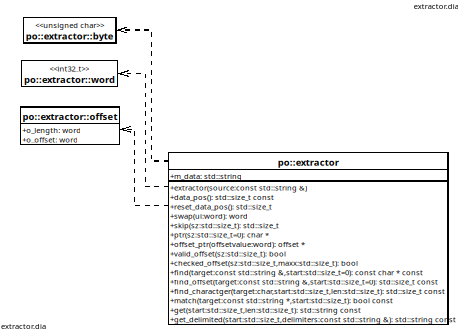
\includegraphics[scale=0.5]{extractor.png}
   \caption{Binary Data Extractor (po::extractor)}
   \label{fig:potext_extractor}
\end{figure}

   For the most part, the data in the string is accessed by position and
   length. Offsets and pointers for string or character targets can be
   found using a starting offset, a length, and perhaps a character delimiter
   such as a newline, null byte, and the EOT (ASCII 4) character.

   Note the data types of \texttt{byte} and \texttt{word}, here hidden in the
   extractor class.

   Also included is the \texttt{offset} structure, which is the pair of data
   items the \texttt{.mo} format uses.

\subsection{Dictionary Class}
\label{subsec:potext_dictionary_class}

   The \texttt{po::dictionary} class is a reimplementation of the
   \texttt{tinygettext::Dictionary} class.

\begin{figure}[H]
   \centering 
   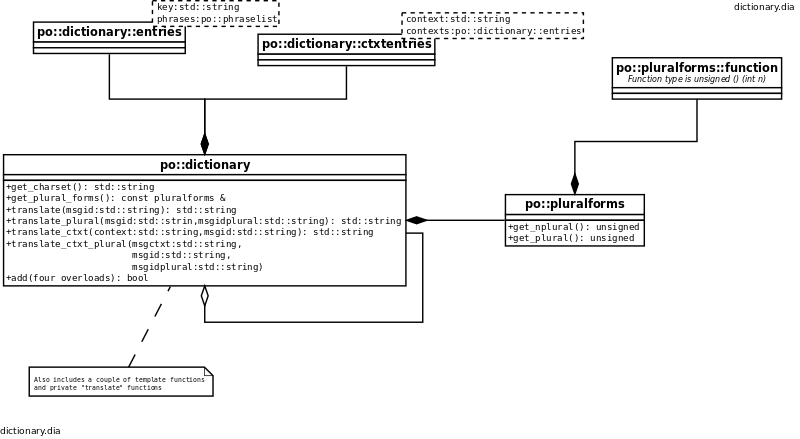
\includegraphics[scale=0.80]{dictionary.png}
   \caption{Dictionary (po::dictionary)}
   \label{fig:potext_dictionary}
\end{figure}

   The \texttt{dictionary} class holds a set of conversions of strings to a
   list of possible conversions, and another set of lists to support various
   message contexts.

   The dictionary contains \texttt{entries}, an \texttt{std::unordered\_map}
   of phrases keyed by a message ID string as used in \textsl{GNU}
   \texttt{gettext()}.
   A \texttt{phraselist} is simply an \texttt{std::vector<std::string>}.

   The dictionary also contains \texttt{ctxtentries},
   an \texttt{std::unordered\_map} of \texttt{entries} keyed by a
   context string.

   The dictionary also contains a \texttt{pluralforms} object that can be used
   to look up the proper plural translation.
   These functions provide the desired lookups:

   \begin{itemize}
      \item \texttt{translate()}. 
      \item \texttt{translate\_plural()}. 
      \item \texttt{translate\_ctxt()}. 
      \item \texttt{translate\_ctxt\_plural()}. 
   \end{itemize}

   Note that there are no functions that use the name of a domain as
   a parameter.
   Instead, the domain-using functions in the \texttt{gettext} module
   look up the dictionary associated with the desired domain, 
   and use the appropriate translate function.

   The \texttt{pluralforms} class deserves its own small section.

\subsection{Pluralforms Class}
\label{subsec:potext_pluralforms_class}

   The \texttt{po::pluralforms} class is a reimplementation of the
   \texttt{tinygettext::PluralForms} class.
   Each \texttt{.po} file contains a line describing how the translation of
   plurals is to be handled for each language:

   \begin{verbatim}
      Plural-Forms: nplurals=2; plural=n != 1;
   \end{verbatim}
   
   The \texttt{pluralforms} class provides a static function for each
   possible plural form (and there are quite a number of them).
   These functions are inserted into an \texttt{std::unordered\_map}
   which is keyed by strings like the one shown above.
   Some of these strings are extremely long.
   \textsl{(We could shorten the keys by ignoring the redundant part
   of the plural-forms string.)}

   The \texttt{po::pluralforms::from\_string()} function strips the
   spaces from a string parameter and does a fast lookup to return the
   appropriate \texttt{pluralforms} object.

\subsection{Language Class}
\label{subsec:potext_language_class}

   The \texttt{po::language} class is a reimplementation of the
   \texttt{tinygettext::Language} class.

   The \texttt{po::languagespec} structure is a reimplementation of the
   \texttt{tinygettext::LanguageSpec} structure.
   This structure now uses \texttt{std::string} instead of character pointers.

\begin{figure}[H]
   \centering 
   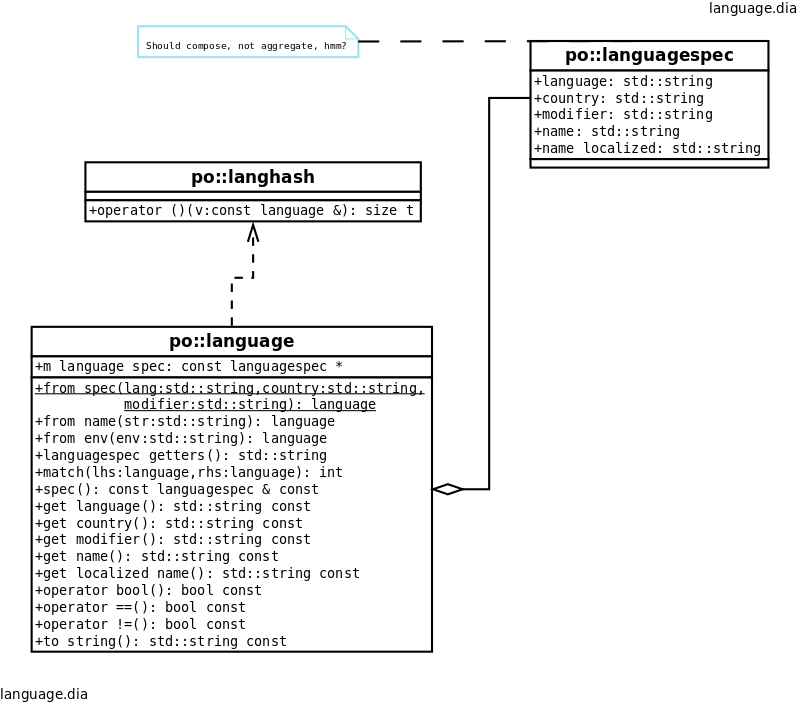
\includegraphics[scale=0.75]{language.png}
   \caption{Language (po::language)}
   \label{fig:potext_language}
\end{figure}

   The \texttt{language} class is a wrapper for a
   \texttt{languagespec} structure.
   As shown in the figure, it provides functions to get and set the
   components of a language specification, to make comparisons, and
   converted the specification to a string.

   The \texttt{dictionarymgr} uses the
   \texttt{language} as a key to look up the desired dictionary, and
   if not found, to make a new dictionary and add it to the dictionary
   container.

% TODO
   We still need to understand a little more about this class and its usage.
% TODO

\subsection{NLS Bindings Class}
\label{subsec:potext_nlsbindings_class}

   The \texttt{nlsbindings} class is an addition for the \textsl{Potext}
   library to support adding text-domain functions akin to those in
   \textsl{GNU Gettext}, but wrapped in the \texttt{po} namespace.

\begin{figure}[H]
   \centering 
   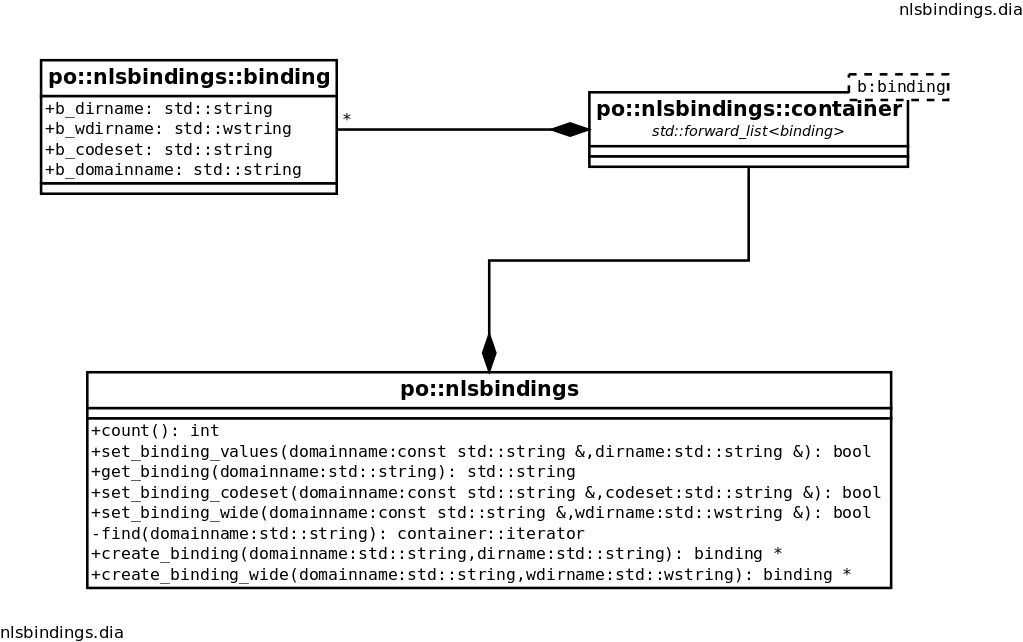
\includegraphics[scale=0.9]{nlsbindings.png}
   \caption{NLS Bindings (po::nlsbindings)}
   \label{fig:nlsbindings}
\end{figure}

   It provides some simplified implementations of
   \textsl{GNU Gettext} functions that lack such niceties as
   locking and checking for SUID root applications.
   These can be added later as the need becomes apparent.
   For details, see the code in the 
   \textsl{GNU Gettext} project in it's
   \texttt{gettext-runtime/intl} directory.

\subsection{Gettext Module}
\label{subsec:potext_gettext_module}

   The \textsl{Potext} \texttt{gettext} module is discussed in the next
   section.
   (See \sectionref{subsec:gettext_module}.)

%-------------------------------------------------------------------------------
% vim: ts=3 sw=3 et ft=tex
%-------------------------------------------------------------------------------

%-------------------------------------------------------------------------------
% gettext
%-------------------------------------------------------------------------------
%
% \file        gettext.tex
% \library     Documents
% \author      Chris Ahlstrom
% \date        2024-02-15
% \update      2024-03-22
% \version     $Revision$
% \license     $XPC_GPL_LICENSE$
%
%     Provides a description of the modified gettext.h header file and
%     the gettext module that reimplements parts of it.
%
%-------------------------------------------------------------------------------

\section{GNU Gettext and Its Potext Replacements}
\label{subsec:gettext_code}

   This section briefly covers the public functions and macros of
   \textsl{GNU Gettext} and our replacements for them.
   Here are the main differences:

   \begin{itemize}
      \item All implementations are functions; no macros are used.
      \item All functions are inside the \texttt{po} namespace.
      \item All character pointers are replaced by \texttt{std::string}.
      \item Lookups are done via \texttt{.po} files, at present.
      \item None of the functions with a "category" parameter are
         implemented at this time.
         Those function would seem to need to find an load up another
         \texttt{dictionary} object.
         Also, by far the most common translation files on a \textsl{UNIX}
         system are in the \texttt{LC\_MESSAGE} subdirectories.
   \end{itemize}

\subsection{GNU Gettext Header File}
\label{subsec:gettext_gnu_header_file}

   This section provides a walkthrough of the \texttt{gettext.h} header file
   of the \textsl{Potext} library.
   This is useful in understanding \textsl{Gettext} versus \textsl{Potext}.

   Let us survey the important functions and macros that are used in
   the \texttt{gettext.h} header file
   (see \texttt{/usr/include/libintl.h}):

   \begin{itemize}
      \item \texttt{ENABLE\_NLS}.
         If defined in a GNU automake project, this includes the
         \texttt{libintl.h} header file, which is not needed in
         an application using the \textsl{Potext} library for translation.
         NLS can be disabled via \texttt{--disable-nls}.
      \item \texttt{DEFAULT\_TEXT\_DOMAIN}.
         If \texttt{ENABLE\_NLS} is defined, this macro causes
         \texttt{gettext} to be defined as \texttt{dgettext}, and
         \texttt{ngettext} to be defined as \texttt{dngettext}.
         If \texttt{ENABLE\_NLS} is \textsl{not} defined, then the following
         "functions" are "voided":
         \begin{itemize}
            \item \texttt{gettext}
            \item \texttt{dgettext}
            \item \texttt{dcgettext}
            \item \texttt{ngettext}
            \item \texttt{dngettext}
            \item \texttt{dcngettext}
            \item \texttt{textdomain}
            \item \texttt{bindtextdomain}
            \item \texttt{bind\_textdomain\_codeset}
         \end{itemize}
      \item \texttt{DEFAULT\_TEXT\_DOMAIN} revisited.
         If defined, more macros are defined, for message-context support.
         These call \texttt{pgettext\_aux}
         or \texttt{npgettext\_aux}
         \begin{itemize}
            \item \texttt{pgettext}
            \item \texttt{dpgettext}
            \item \texttt{dcpgettext}
            \item \texttt{npgettext}
            \item \texttt{dnpgettext}
            \item \texttt{dcnpgettext}
         \end{itemize}
      \item \texttt{GNULIB\_defined\_setlocal}.
         If defined, uses the \texttt{rpl\_setlocale} from \textsl{gnulib}
         as \texttt{setlocale}.
      \item \texttt{gettext\_noop}.
         A pseudo function that marks code for extraction of messages, but
         does not call \texttt{gettext}.
      \item \texttt{pgettext\_expr}. Calls \texttt{dcpgettext\_expr()}.
      \item \texttt{dpgettext\_expr}. Calls \texttt{dcnpgettext\_expr()}.
   \end{itemize}

   Do we want \textsl{potext} to be a drop-in replacement for all this stuff?
   We shall try!

\subsection{Gettext Module}
\label{subsec:gettext_module}

   The \texttt{gettext} module provides a reimplementation of
   \textsl{GNU Gettext} "gettext" functions in the \texttt{po}
   namespace.

   Here, we use the term "module" to describe a set of related functions
   that are not members of a class.
   All functions in this module are in the \texttt{po}
   namespace, or are \texttt{static} and internal to the module.

\begin{figure}[H]
   \centering 
   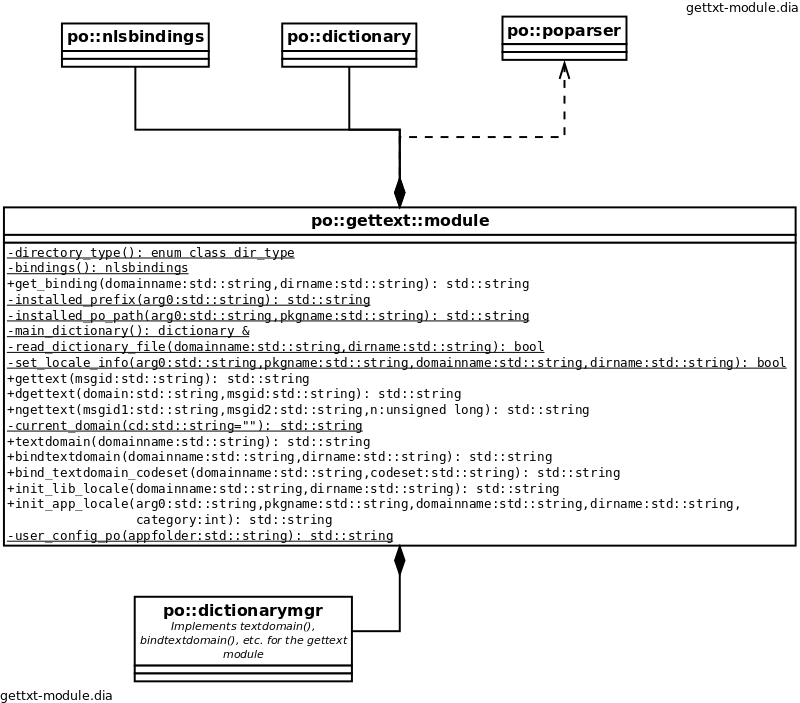
\includegraphics[scale=0.75]{gettext-module.png}
   \caption{Gettext Module (namespace po)}
   \label{fig:gettext_module}
\end{figure}

   We are slowly implement the various "gettext" functions shown in that
   figure, plus some others that are not shown.
   See the next section for a brief discussion of our copy of the
   \texttt{GNU Gettext} header file.

   The following table lists the functions/macros and their purpose and status.
   The implementations are member functions of
   \texttt{po::dictionary} or
   \texttt{po::dictionarymgr} (*); all dictionaries are contained and
   referenced in \texttt{po::dictionarymgr}, either as the main dictionary
   or a dictionary selected based on domain.
   Fall-back functions are noted for some "none" implementations.

   \begin{table}[H]
      \centering
      \caption{Gettext Functions}
      \label{table:potext_gettext_functions}
      \resizebox{\textwidth}{!}{%
      \begin{tabular}{l l p{7cm}}

         \textbf{Function} & \textbf{Implementation} & \textbf{Purpose} \\

         \texttt{textdomain()} & textdomain() * &
            Set or change the current global domain for the
            \texttt{LC\_MESSAGE} category. \\

         \texttt{bindtextdomain()} & bindtextdomain() * &
            Set or change the locale directory for the given domain.
            \texttt{LC\_MESSAGE} category.
            The wide-character \texttt{UTF-16} version for \textsl{Windows}
            is not yet implemented. \\

         \texttt{bind\_textdomain\_codeset()} & partial * &
            Set or change the character-set for the given domain.
            \texttt{LC\_MESSAGE} category. \\

         \texttt{gettext()} & translate() &
            Single message ID translation. \\

         \texttt{dgettext()} & translate() &
            Single message ID translation in a specific domain. \\

         \texttt{dcgettext()} & none: dgettext() &
            Single message ID translation in a specific domain
            and specific language category.
            For all get-text functions with a category parameter,
            there is currently no implementation, just a fall-back
            to the non-category version.\\

         \texttt{ngettext()} & translate\_plural() &
            Message ID translation using a specific singular
            or plural form. \\

         \texttt{dngettext()} & translate\_plural() &
            Message ID translation using a specific singular
            or plural form for a given domain. \\

         \texttt{dcngettext()} & none: translate\_plural()&
            Message ID translation using a specific singular
            or plural form for a given domain and a given locale
            category. \\

         \texttt{pgettext()} & translate\_ctxt() &
            Single message ID translation for a given context (e.g.
            "console" versus "gui". The 'p' stands for 'particular'.\\

         \texttt{dpgettext()} & translate\_ctxt() &
            Single message ID translation for a given context and the
            given domain. \\

         \texttt{dpcgettext()} & none: dpgettext() &
            Single message ID translation for a given context,
            given domain, and category
            other than \texttt{LC\_Messages}. \\

         \texttt{npggettext()} & no &
            Probaby worth doing. \\

         \texttt{dnpggettext()} & no &
            Probaby worth doing. \\

         \texttt{dcnpggettext()} & no &
            Probaby not worth doing. \\

      \end{tabular}}
   \end{table}

%-------------------------------------------------------------------------------
% vim: ts=3 sw=3 et ft=tex
%-------------------------------------------------------------------------------

%-------------------------------------------------------------------------------
% tests
%-------------------------------------------------------------------------------
%
% \file        tests.tex
% \library     Documents
% \author      Chris Ahlstrom
% \date        2024-02-09
% \update      2024-04-07
% \version     $Revision$
% \license     $XPC_GPL_LICENSE$
%
%     Provides a pointed description of some tests, which also helps understand
%     usage of the potext library, a replacement for the tinygettext library..
%
%-------------------------------------------------------------------------------

\section{Potext Tests}
\label{sec:potext_tests}

   This section provides a useful walkthrough of the testing
   of the \textsl{potext} library.
   They illustrate the various way in which the \textsl{Potext} library
   can be used by a develper.

   These tests are not installed; they are in the transitory
   directory \texttt{potext/build/library/tests}.
   The test \texttt{*.po} files are in the 
   directory \texttt{potext/library/tests} and its subdirectories.
   The shell script
   \texttt{library/tests/tests.sh} runs all of the
   \texttt{potext\_test} tests listed in the following file,
   plus a couple more.

   \begin{verbatim}
      library/tests/testlines.list
   \end{verbatim}

   It specifies the tests
   described here, but using only single-word phrases.
   The reason is that we have not yet figured out how to deal
   with phrases enclosed in double-quotes in a shell script.

   Let us survey the main features of all of the test \texttt{po}
   files:

   \begin{itemize}
      \item \texttt{po} directory.
         This directory contains a small sampling of \texttt{.po}
         files from the \textsl{GNU Gettext} project.
         They have been pared down a bit just to save a few bytes,
         and a few extra translations have bee added for testing.
         They are used in the new
         \texttt{hellopotext} test program to
         test the functions in the \texttt{gettext} C++ module.
      \item \texttt{library/tests/de.po}.
         A basic \texttt{po} file with just
         \texttt{msgid} keys and
         \texttt{msgstr} translations in Deutsche (German, Alemania).
      \item \texttt{library/tests/broken.po}.
         This file has an entry \texttt{msgstr[10]}, obviously bad.
      \item \texttt{library/tests/helloworld/de.po}.
         It has some \texttt{msgctxt} sections with
         \texttt{msgid\_plural},
         \texttt{msgstr[0]} for a singular translation and
         \texttt{msgstr[1]} for a plural translation 
         for each context (none, "gui", and "console").
      \item \texttt{library/tests/level/de.po}.
         Contains basic entries plus a number of entries with a blank
         message-ID followed by a long description and a message-string
         with a blank value followed by a long translation.
         NEED TO FIGURE THAT OUT.
         Also includes a couple of \texttt{printf()} format statements.
      \item \texttt{library/tests/po/de.po}.
         Another basic file with a number of translations and a
         weird message-ID called "umlaut".
      \item \texttt{library/tests/po/de\_AT.po}.
         A short file with "umlaut" and a couple of plurals.
      \item \texttt{library/tests/po/fr.po}.
         Contains one German translation. Wtf?
   \end{itemize}

   One thing to watch for in running the tests.
   The test programs write output to \texttt{std::cout} or
   \texttt{std::cerr}, while the \textsl{Potext} library
   internals use the \texttt{po::logstream} class functions.
   What happen is the all of the application output comes first,
   while the log-stream message are not emitted until
   test program exit.
   Not sure why the latter aren't "flushed" immediately.

   Here are the tests provided:

    \begin{itemize}
        \item \texttt{helloworld}
        \item \texttt{hellopotext}
        \item \texttt{po\_parser\_test}
        \item \texttt{mo\_parser\_test}
        \item \texttt{potext\_test}
    \end{itemize}

   The code is in the \texttt{library/tests} directory, and the
   executables are written to \texttt{build/library/tests}
   directory.

\subsection{Hello World}
\label{subsec:potext_hello_world}

   \texttt{helloworld}.
   This test is the original from the \textsl{tinygettext} project.
   Not much done with it; it includes a copy of the
   \texttt{gettext.h} header file and calls some of the stock
   \textsl{GNU Gettext} functions.

\subsection{Hello Potext}
\label{subsec:potext_hello_potext}

   \texttt{hellopotext}.
   This application is a good test of \textsl{potext} from the
   perspective of a developer wanting to use it in an application.
   Without arguments, this test runs through basic tests of the following
   functions.
   The main domain is provided to \texttt{po::init\_app\_locale()}
   which should normally be called in the applications's
   \texttt{main()} entry point function.

   \begin{itemize}
      \item \texttt{\_()} and \texttt{gettext()}.
         This function does a message translation lookup using
         the current domain, which is logged in the
         \texttt{init\_app\_locale()} function.
         This smoke test illustrates the most common case we want to
         cover, which is the translation of a phrase according to
         the main (or only) domain and locale directory loaded.
         Also included is a test where the original message is not
         present in the \texttt{.po} file.
      \item \texttt{dgettext}.
         This function looks up a domain's dictionary and uses it
         for the translation.
         This test runs through all of the domains (i.e. \texttt{.po}
         files) in the \texttt{po} project directory.
         Currently tested are the \textsl{es}, \textsl{fr}, \textsl{de},
         and a bogus domain named \textsl{xx}, which should just return
         the input message ID.
      \item \texttt{dcgettext}.
         This test does not do anything.
         Currently \textsl{Potext} does not handle locale categories.
         The reasons? First, the most common use case is looking up
         message translations in the \texttt{LC\_MESSAGES} locale category.
         Second, this translation would require loading additional locale
         directories and their dictionaries.
         With this complication, we will sit on this problem for awhile.
      \item \texttt{ngettext}.
         This test handles plural forms in the current domain.
         It deals only the the main domain, \texttt{es},
         It tests translating the plurals of the following singulars:
         "File" and "Person". 
         The translations are likely not accurate, as they were provided
         by \textsl{Google Translate}.
         But they adequately test the process.
      \item \texttt{dngettext}.
         This test handles plural forms in a specified domain.
         Currently tested are the \textsl{es}, \textsl{fr}, \textsl{de},
         and a bogus domain named \textsl{xx}, which should just return
         the input message ID.
      \item \texttt{dcngettext}.
         This function is not yet implemented, due to difficulties
         with selecting the category directory, as discussed above.
      \item \texttt{pgettext}.
         This test applies only to the domain specified in the
         \texttt{init\_app\_locale()} function.
   \end{itemize}

   Some functions not yet tested because of the implmentation difficulties
   noted above.

   \begin{itemize}
      \item \texttt{dcgettext()}.
      \item \texttt{dcngettext()}.
   \end{itemize}

   Additional arguments can change the default domain.
   We will document these \textsl{real soon now}.

\subsection{PO Parser Test}
\label{subsec:potext_Po_parser_test_program}

   \texttt{po\_parser\_test}
   This small application tests the ability to parse some
   sample \texttt{.mo} files.

   To run this test, simply supply the name of a \texttt{.po} file and
   examine the results.
   Any \texttt{.po} file can be provided.

   Without arguments, this application lists some options and stock
   test \texttt{.po} files to run.

\subsection{MO Parser Test}
\label{subsec:potext_mo_parser_test_program}

   \texttt{mo\_parser\_test}
   This small application tests the ability to parse some
   sample \texttt{.mo} files.

   To run this test, simply supply the name of a \texttt{.mo} file and
   examine the results.
   Any \texttt{.mo} file can be provided.

   Without arguments, this application lists some options and stock
   test \texttt{.mo} files to run.

   In progress.
   We need to add some more files to be able to test all of the most
   important aspects of \texttt{.mo} files.

\subsection{Potext Test}
\label{subsec:potext_test_program}

   \texttt{potext\_test}
   This application is another good test of \textsl{potext} from the
   perspective of a developer wanting to use it in an application.
   Running it without any arguments shows a list of 8 tests.
   These tests are run by supplying the appropriate command-line arguments.
   These are reflected in the following sections.

\subsubsection{Potext Test 'Translate'}
\label{subsubsec:potext_test_translate}

   These tests are run using a command like the following:

   \begin{verbatim}
      $ ./build/library/tests/potext_test translate <...options...>
   \end{verbatim}

   By running \texttt{potext\_test} without any options, one sees
   four "translate" commands.
   The four variations on the "translate"
   test are described in the following sub-sections.

\paragraph{Translate Basic: Po File and Sample Message}
\label{paragraph:potext_test_translate_po_message}

   This test is a simple translation of a word.
   The basic "translate" test is run by the following form, which has an
   argument count of 4.

   \begin{verbatim}
      $ ./build/library/tests/potext_test translate <file> <msg>
   \end{verbatim}

   The file is a test \texttt{.po} file in the
   \texttt{tests} directory.
   The message is a phrase present in that file, such as
   \textsl{"F1 - show/hide this help screen"}, translated in
   \texttt{de.po} as
   \textsl{"F1 - Hilfe anzeigen/verstecken"}.

   Here is the run:

   \begin{verbatim}
      $ ./build/library/tests/potext_test translate \
         library/tests/de.po "F1 - show/hide this help screen"
   \end{verbatim}

   The output is

   \begin{verbatim}
      Translation: "F1 - Hilfe anzeigen/verstecken"
   \end{verbatim}

   If only a part of the message is provided, of course there is no
   match, and the message is

   \begin{verbatim}
      Translation: "F1 - Hilfe"
      [potext] Couldn't translate: "F1 - Hilfe"
   \end{verbatim}

   This second test shows that any deviation from a supported message causes an
   warning, and returns the original message.
   These deviations include missing letters, missing punctuation,
   additional spaces.
   \textsl{We wonder if we can work around such issues in this library.
   We shall see.}

\paragraph{Translate: Po File, Context, and Sample Message}
\label{paragraph:potext_test_translate_po_context_message}

   This test is run by the following form, which has an argument count
   of 5.

   \begin{verbatim}
      $ ./build/library/tests/potext_test translate <file> <context> <msg>
   \end{verbatim}

   This test requires a \texttt{po} file with message-context
   entries such as these three different entries found in
   \texttt{library/test/helloworld/de.po} for the phrase
   "Hello World":

   \begin{verbatim}
      msgctxt ""
      msgid "Hello World"
      msgctxt "console"
      msgid "Hello World"
      msgctxt "gui"
      msgid "Hello World"
   \end{verbatim}

   Please note that the \textsl{GNU} \texttt{gettext()} documentation says
   that an empty message context (\texttt{msgctxt ""}) is \textsl{not}
   the same as a missing message context.
   In the "helloworld" test program, these contexts are provided by the
   following lines:

   \begin{verbatim}
      pgettext("", "Hello World")
      pgettext("console", "Hello World")
      pgettext("gui", "Hello World")
   \end{verbatim}

   The macros \texttt{ngettext} and \texttt{npgettext} are also used to provide
   access to the various plural forms in that \texttt{po} file.
   In any case, we need to use 
   \texttt{library/test/helloworld/de.po} for this test.
   An actual test run:

   \begin{verbatim}
      $ ./build/library/tests/potext_test translate \
            library/tests/helloworld/de.po "console" "Hello World"
   \end{verbatim}

   The output is

   \begin{verbatim}
      Context 'console' translation: "Hallo Welt (singular) in der Console"
   \end{verbatim}

   If the \texttt{<context>} parameter is not found in the \texttt{po}
   file, a message is emitted to indicate the error.

\paragraph{Translate: Po File with Singular and Plurals}
\label{paragraph:potext_test_translate_po_singular_plural}

   This test is run by the following form, which has an argument count
   of 6.

   \begin{verbatim}
      $ ./build/library/tests/potext_test translate <file> <singular>
            <plural> <N>
   \end{verbatim}

   The singular and plural parameters are message IDs, such as "Hello World".
   This command is a bit tricky; the N value is not a C index, but an
   index that starts at 1.
   The N parameter ranges from 1 to the last array value in
   the \texttt{po} file.
   The number of singular/plural translations depends on the language and
   is specified in the specific \texttt{.po} file using
   a header declaration such as
   \texttt{"Plural-Forms: nplurals=2; plural=(n != 1);"}.
   Look at \texttt{pluralforms.cpp} to see all the plural-forms settings and
   "callbacks" that are support.
   Some of these forms support Slavic and Arabic languages, and we are not able
   to test them.

   An actual test run:

   \begin{verbatim}
      $ ./build/library/tests/potext_test translate \
            library/tests/helloworld/de.po "Hello World" "Hello Worlds" 1
   \end{verbatim}

   The output is

   \begin{verbatim}
      TODO
   \end{verbatim}

\paragraph{Translate: Po File with Context, Singular, and Plurals}
\label{paragraph:potext_test_translate_po_context_singular_plural}

   This test is run by the following form, which has an argument count
   of 7.

   \begin{verbatim}
      $ ./build/library/tests/potext_test translate <file> <context> \
         <singular> <plural> <N>
   \end{verbatim}

   An actual test run:

   \begin{verbatim}
      $ ./build/library/tests/potext_test translate \
            library/tests/helloworld/de.po "gui" "Hello World" "Hello Worlds" 0
   \end{verbatim}

   The output is

   \begin{verbatim}
      TODO
   \end{verbatim}

\subsubsection{Potext Test 'Directory'}
\label{subsubsec:potext_test_directory}

   These tests are run using a command like the following:

   \begin{verbatim}
      $ ./build/library/tests/potext_test directory <dir> <msg> [<lang>]
   \end{verbatim}

\subsubsection{Potext Test 'Language'}
\label{subsubsec:potext_test_language}

   These tests are run using a command like the following:

   \begin{verbatim}
      $ ./build/library/tests/potext_test language <lang>
   \end{verbatim}

\subsubsection{Potext Test 'Language Directory'}
\label{subsubsec:potext_test_language_directory}

   These tests are run using a command like the following:

   \begin{verbatim}
      $ ./build/library/tests/potext_test language-dir <dir>
   \end{verbatim}

\subsubsection{Potext Test 'List Message Strings'}
\label{subsubsec:potext_test_list_message_strings}

   These tests are run using a command like the following:

   \begin{verbatim}
      $ ./build/library/tests/potext_test list-msgstrs <file>
   \end{verbatim}

%-------------------------------------------------------------------------------
% vim: ts=3 sw=3 et ft=tex
%-------------------------------------------------------------------------------


\section{Summary}
\label{sec:summary}

   Contact: If you have ideas about \textsl{Potext} or a bug report,
   please email us (at \url{mailto:ahlstromcj@gmail.com}).

   Remaining issues:

   The \texttt{*.po} files "msgid" and "msgstr" entries have punctuation marks
   and trailing spaces that are significant.
   CAN WE GET AROUND THIS ISSUE?
   We need to trim these trailing characters in both specifications,
   and also when translating, and restore them in the translation.

% References

%-------------------------------------------------------------------------------
% references
%-------------------------------------------------------------------------------
%
% \file        references.tex
% \library     Documents
% \author      Chris Ahlstrom
% \date        2024-03-08
% \update      2024-04-07
% \version     $Revision$
% \license     $XPC_GPL_LICENSE$
%
%     Provides the References section of the Potext manual. Rather
%     than use the bibtex package, our small set of references uses a
%     simpler method.
%     WRK
%
%-------------------------------------------------------------------------------

\section{References}
\label{sec:references}

   The \textsl{Potext} reference list.

{\RaggedRight
\begin{thebibliography}{99}

   \bibitem{gettextcode}
   GNU Translation Team.
   \emph{GNU Gettext Code}
	\url{https://git.savannah.gnu.org/git/gettext.git}.
   2023.

   \bibitem{gettextman}
   GNU Translation Team.
   \emph{GNU Gettext Tools manual, version 0.22.}
   \url{https://www.gnu.org/software/gettext/manual/gettext.pdf}.
   2023.

   \bibitem{simplegettext}
   Laurent Cozic
   \emph{Simple Gettext on GitHub.}
   \url{https://github.com/laurent22/simple-gettext}.
   2017.

   \bibitem{tinygettext}
   Tinygettext Team.
   \emph{Tinygettext on GitHub.}
   \url{https://github.com/tinygettext/tinygettext}.
   2023.

\end{thebibliography}
}

%-------------------------------------------------------------------------------
% vim: ts=3 sw=3 et ft=tex
%-------------------------------------------------------------------------------


\printindex

\end{document}

%-------------------------------------------------------------------------------
% vim: ts=3 sw=3 et ft=tex
%-------------------------------------------------------------------------------
